\subsection{Reduced Order Observer Design}

In general an observer is utilized in a control system if either one of two specific cases occurs. If certain states in the system is not measured, an observer can be utilized to estimate the unmeasured states by utilizing the system output, thus utilizing the states which has been measured. However, it is also possible to use an observer if the measured data gathered from the sensors is affected by noise. The observer can thereby use both the noisy measured states and the estimated states creating a filtered version of the noisy states. This case will however not be utilized in the prototype.

In the attitude control an reduced order observer is used. As written in ?? the attitude model has six states, the three angles of the quadcopter (roll, pitch and yaw) and the three corresponding angular velocities. By using the Vicon system, see ??, the three angles of the quadcopter is measured. Thus making it possible to only estimate the angular velocities with a reduced order observer. 

\begin{figure}[H]
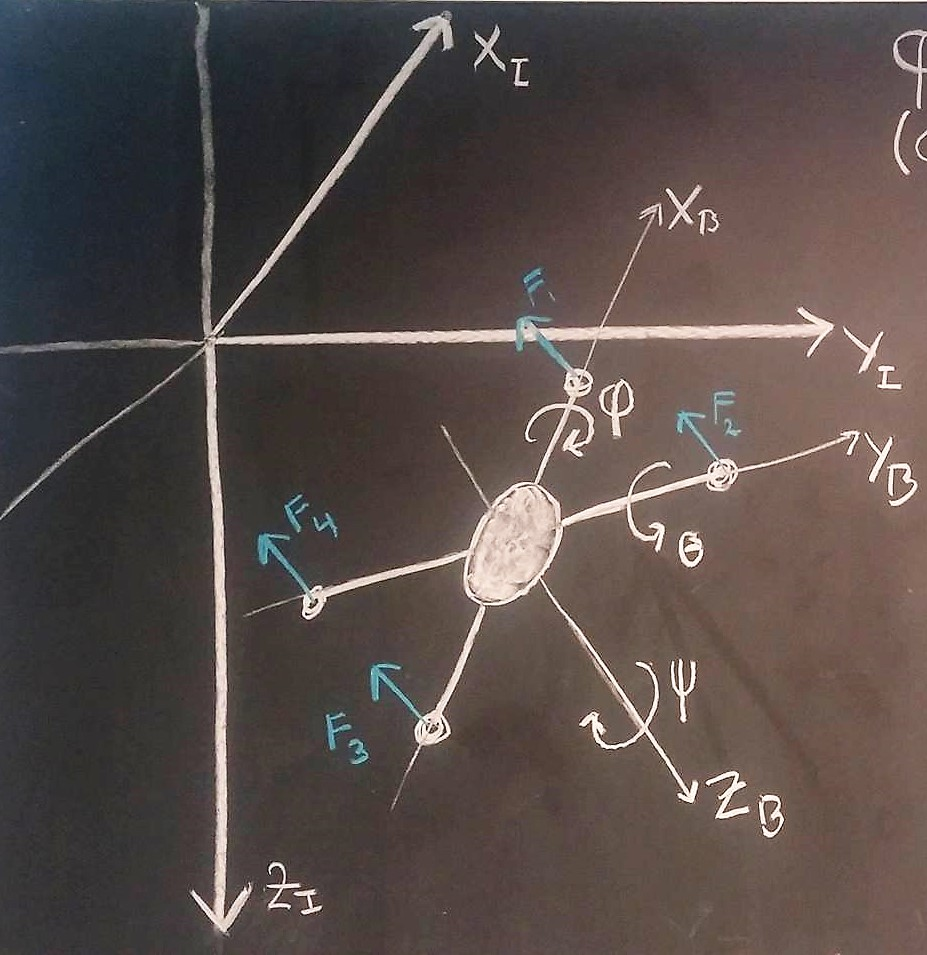
\includegraphics[scale=.27]{figures/drone_diagram}
\centering
\captionsetup{justification=centering}
\captionof{figure}{Diagram of the quadcopter which includes inertial and body reference systems, as well as the references for the angles (roll, pitch and yaw) and the thrust forces produced by the propeller. }
\label{diagramQuad}
\end{figure}

Explain what is it\\
	What is an observer?\\
	
	What is an reduced order observer?\\
Diagram with colors + Block diagram\\
Equations\\
Simulation??\\



\begin{flalign}  \label{observability}
	\vec{{\mathcal O}} = 
	\begin{bmatrix}
		\vec{C} \\
		\vec{C}\vec{A} \\
		\vec{C}\vec{A}^2 \\
		\vec{C}\vec{A}^3 \\
		\vec{C}\vec{A}^4 \\
		\vec{C}\vec{A}^5 \\		
	\end{bmatrix}
	\si{=}
	\begin{bmatrix}
		\ \ 1 & 0 & 0 & 0 & 0 & 0 \ \ \\
		\ \ 0 & 1 & 0 & 0 & 0 & 0 \ \ \\
		\ \ 0 & 0 & 1 & 0 & 0 & 0 \ \ \\
		\ \ 0 & 0 & 0 & 1 & 0 & 0 \ \ \\
		\ \ 0 & 0 & 0 & 0 & 1 & 0 \ \ \\
		\ \ 0 & 0 & 0 & 0 & 0 & 1 \ \ \\
		\ \ 0 & 0 & 0 & 0 & 0 & 0 \ \ \\
		\ \ 0 & 0 & 0 & 0 & 0 & 0 \ \ \\
		\ \ 0 & 0 & 0 & 0 & 0 & 0 \ \ \\
		\ \ 0 & 0 & 0 & 0 & 0 & 0 \ \ \\
		\ \ 0 & 0 & 0 & 0 & 0 & 0 \ \ \\
		\ \ 0 & 0 & 0 & 0 & 0 & 0 \ \ \\
		\ \ 0 & 0 & 0 & 0 & 0 & 0 \ \ \\
		\ \ 0 & 0 & 0 & 0 & 0 & 0 \ \ \\
		\ \ 0 & 0 & 0 & 0 & 0 & 0 \ \ \\
		\ \ 0 & 0 & 0 & 0 & 0 & 0 \ \ \\
		\ \ 0 & 0 & 0 & 0 & 0 & 0 \ \ \\
		\ \ 0 & 0 & 0 & 0 & 0 & 0 \ \ 														
	\end{bmatrix}
\end{flalign}

\begin{figure}[H]
	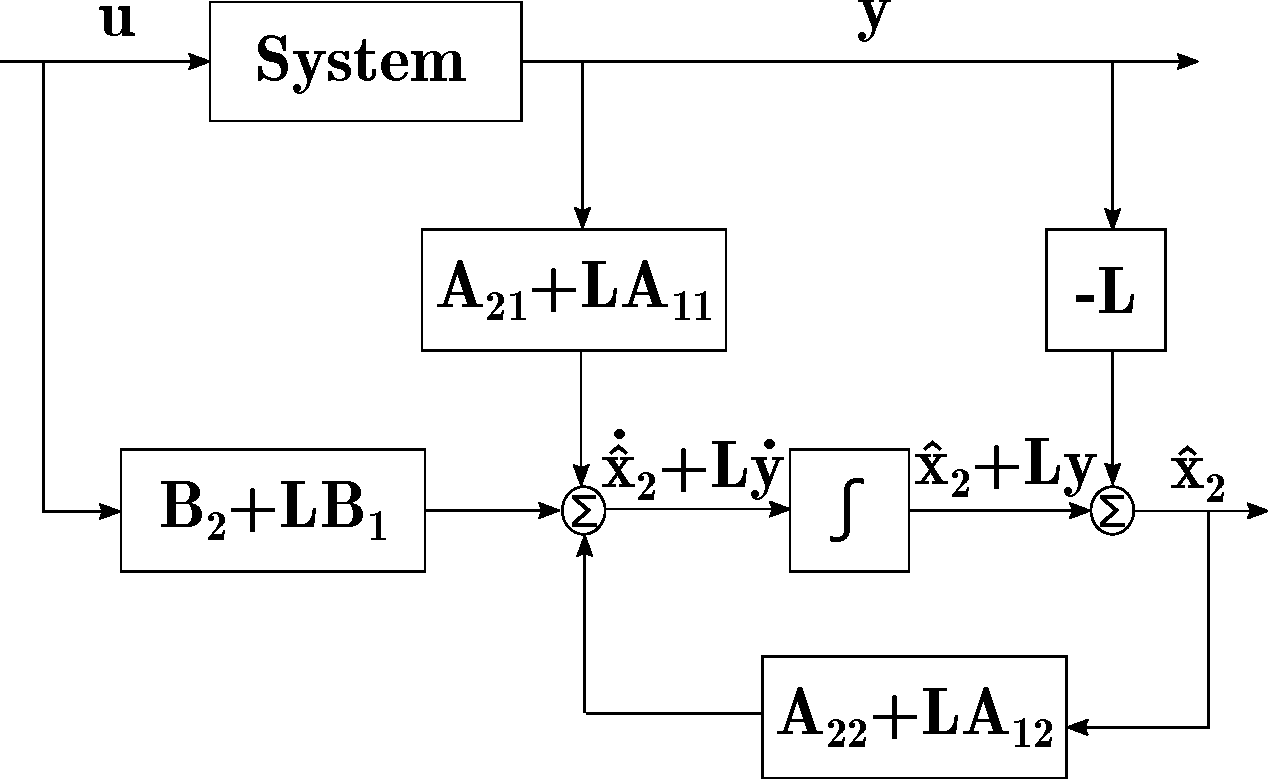
\includegraphics[scale=.35]{figures/observerDiagram}
	\centering
	\captionsetup{justification=centering}
	\captionof{figure}{Diagram . }
	\label{observerDiagram}
\end{figure}


\begin{minipage}{0.15\linewidth}
	\begin{flalign}
	A_{11} = 
	\begin{bmatrix}
		\ 0 & 0 & 0 \ \ \\ 
		\ 0 & 0 & 0 \ \ \\ 
		\ 0 & 0 & 0 \ \ \\
	\end{bmatrix}	\nonumber
	\label{A11}
	\end{flalign}  
\end{minipage}\hfill
\begin{minipage}{0.15\linewidth}
	\begin{flalign}
	A_{12} = 
	\begin{bmatrix}
		\ 1 & 0 & 0 \ \ \\ 
		\ 0 & 1 & 0 \ \ \\ 
		\ 0 & 0 & 1 \ \ \\
	\end{bmatrix}	\nonumber
	\label{A12}
	\end{flalign}
\end{minipage}\hfill
\begin{minipage}{0.15\linewidth}
	\begin{flalign}
	A_{21} = 
	\begin{bmatrix}
		\ 0 & 0 & 0 \ \ \\ 
		\ 0 & 0 & 0 \ \ \\ 
		\ 0 & 0 & 0 \ \ \\
	\end{bmatrix}	\nonumber
	\label{A21}
	\end{flalign}
\end{minipage}\hfill
\begin{minipage}{0.15\linewidth}
	\begin{flalign}
	A_{22} = 
	\begin{bmatrix}
		\ 0 & 0 & 0 & 0 \ \ \\ 
		\ 0 & 0 & 0 & 0 \ \ \\ 
		\ 0 & 0 & 0 & 0 \ \ \\
	\end{bmatrix} 
	\label{A22}
	\end{flalign}
\end{minipage}\hfill


\begin{minipage}{0.5\linewidth}
	\begin{flalign}
	B_1 = 
	\begin{bmatrix}
		\ 0 & 0 & 0 & 0 \ \ \\ 
		\ 0 & 0 & 0 & 0 \ \ \\ 
		\ 0 & 0 & 0 & 0 \ \ \\
	\end{bmatrix}	\nonumber
	\label{B1}
	\end{flalign}
\end{minipage}\hfill
\begin{minipage}{0.5\linewidth}
	\begin{flalign}
	B_2 = 
	\begin{bmatrix}
		0 & \si{-\frac{2 \cdot k_{th} \cdot L \cdot \overline{\omega}_2}{J_x}} & 0 & \si{\frac{2 \cdot k_{th} \cdot L \cdot \overline{\omega}_4}{J_x}} \ \ \ \\ 
		\ \si{\frac{2 \cdot k_{th} \cdot L \cdot \overline{\omega}_1}{J_y}} & 0 & \si{-\frac{2 \cdot k_{th} \cdot L \cdot \overline{\omega}_3}{J_y}} & 0 \ \ \ \\ 
		\frac{2 \cdot k_d \cdot {\overline{\omega}_1}}{J_z} & - \frac{2 \cdot k_d \cdot {\overline{\omega}_2}}{J_z} & \frac{2 \cdot k_d \cdot {\overline{\omega}_3}}{J_z} & - \frac{2 \cdot k_d \cdot {\overline{\omega}_4}}{J_z} \ \ \
	\end{bmatrix}
	\label{B2}
	\end{flalign}
\end{minipage}\hfill


\begin{flalign}
	L = 
	\begin{bmatrix}
	\ -50 & 0 & 0  \ \ \ \\ 
	\ 0 & -60 & 0  \ \ \ \\ 
	\ 0 & 0 & -70  \ \ \  
	\end{bmatrix}
	\label{Lobs}
\end{flalign}


